\begin{chaptercover}{Exploits}%
{\coverepigraph{``I get hired by companies to hack into their systems and break into their physical facilities to find security holes. Our success rate is 100\%; we've always found a hole."}{\textsc{Kevin Mitnick} \newline {\normalsize\vspace{-.3cm}Cybersecurity consultant}}
{\large \hyphenation{} \bigletter{S}{ystems} have almost always flaws. No \acrshort{is} should ever be considered as completely secure. Even if everything seems to be perfectly hermetic to an attacker, it is always a matter of time before a vulnerability is discovered and the system could be breached. \newline \\ In this chapter, we will put to use the findings discovered in Chapter \ref{scope} in order to exploit the drones in ways unintended by the manufacturer. \newline\\}}%
{exploits}

Now that we have performed our vulnerability analysis, we have a better understanding of how both drones operate. Strong with this knowledge, we will try to gain access or control of them in ways not intended by the manufacturer.

\lstset{
  language=bash,
  backgroundcolor=\color{lightgray},
  showstringspaces=false,
  basicstyle=\ttfamily\color{black},
  commentstyle=\ttfamily\color{black},
  keywordstyle=\ttfamily\color{blue}
}

\section{Flitt Selfie Cam}

This section details a few successful exploits that could be achieved.

\subsection{Telnet attack}

The first possible weakness of the device is the open port TCP/23 allowing telnet connection. Unfortunately, there were no feature in the app that uses the functionality so we were not able to intercept the password nor find it in the code of the APK.

We the decided to give a go to a dictionary attack. It involves testing a series of potential passwords, one after the other, hoping that the password used for encryption is contained in the dictionary. To that end, the first step is to get ourselves a good dictionary. As already presented in Subsection \ref{subsec:hacking-techniques}, the RockYou wordlist is certainly a good choice in terms of completeness as it contains more than 14 million unique passwords and it is shipped with Kali Linux, the distribution we use.

Next is to set up a dictionary attack on a telnet service. To achieve that, we used the Hydra tool (presented in Subsection \ref{subsec:tools-and-resources}). It is fairly simple to use, using the following syntax :

\begin{center}
\begin{minipage}{.95\linewidth}
\begin{lstlisting}
root@kali:~# hydra -l <username> -P <password_file> telnet://targetname
\end{lstlisting}
\end{minipage}
\end{center}

We were confronted to two main issues :
\begin{enumerate}
  \item We had no idea which username is allowed to use the telnet service on the drone side. By default, we tried it with the \texttt{root} account.
  \item The battery of the drone has to be removed in order to be charged and only last for around one hour. It is relatively slow to establish a telnet connection, since it is TCP based, and we were only able to test around 10.000 password each hour before having to pause the attack and recharge the battery.
\end{enumerate}

We proceeded with the attack until we tested around 100.000 passwords, but the odds of a success were considered to low considering the two issues above so we decided to move on.

\subsection{\acrshort{uart} shell access}

This process started with physically opening the device in order to determine the precise hardware in use. Through manual inspection of the device’s internals, it was possible to obtain the relevant component datasheets from the Internet. The chip used in the Flitt Selfie Cam is a Hi3518 \cite{hi3518-datasheet}, which is designed for light video processing, and mostly used in IP cameras. 

Two of the most common relevant interfaces for hardware hacking are \acrfull{uart} and \acrfull{jtag}. \acrshort{jtag} is immensely powerful, usually providing read and write from memory, debugging, extract Firmware, bypass protection mechanisms and more. However, it can be rather difficult to use and requires additional hardware. \acrshort{uart}, on the other hand, is much less powerful but much easier to work with, and usually only uses 2-3 pins (ground, TX and RX). Fortunately, on a lot of IoT devices, an exposed \acrshort{uart} interface is almost always used by the bootloader and OS for a hardware console.

The next step is going to be to identify the different pins that are responsible for the \acrshort{uart} communication. As can be seen on the datasheets, the Hi3518 has 3 sets of \acrshort{uart} pins like presented in Appendix \ref{app:uart-pins}. Our goal here would be to connect to the \acrshort{uart} 0 pins in order to obtain a shell access.

\begin{figure}[H]
\begin{center}
\begin{tabular}{m{9.5cm}m{7.8cm}}
  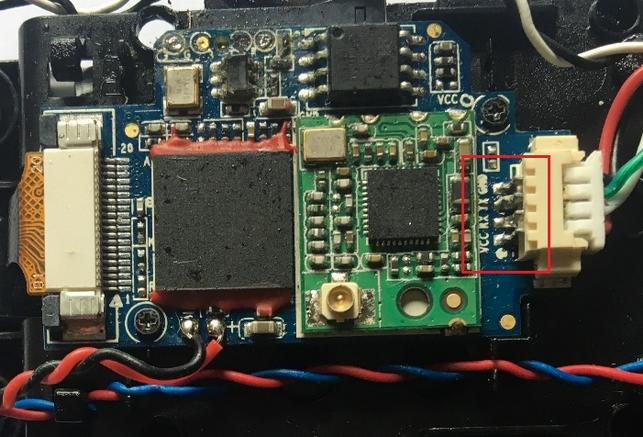
\includegraphics[width=\linewidth]{uart-pins}
  \caption{Bad set of \acrshort{uart} pins of the Flitt Selfie Cam}
  & We could identify a first set of pins rather quickly and proceeded to solder wires on the TX, RX and ground respective pins. Notice that the pins connect to a cable which leads to a second PCB responsible for the control of the 4 motors. It is therefore likely that there are the \acrshort{uart} 1 pins. \\
\end{tabular}
\end{center}
\end{figure}

The procedure was tested using the standard baud rates for serial devices, being 110, 300, 600, 1200, 2400, 4800, 9600, 14400, 19200, 38400, 57600, 115200, 128000 and 256000 bits per second \cite{baudrate}. As it can be seen in Figure \ref{fig:uart-shell-access-failure}, the connection was not successful. 

\begin{figure}[H]
  \centering
  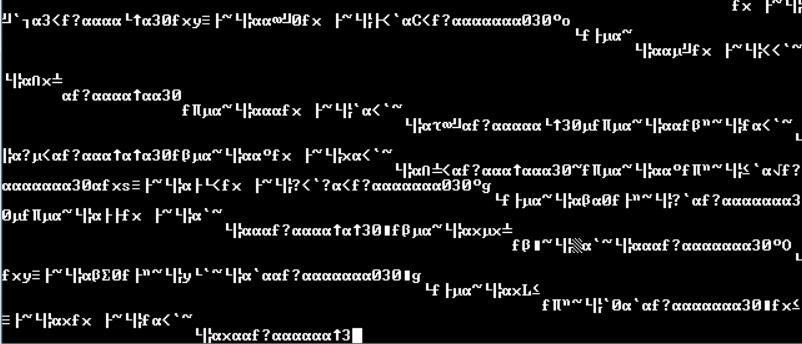
\includegraphics[width=.8\linewidth]{figures/uart-shell-access-failure}
  \caption{Failure in getting shell access through the \acrshort{uart}}
  \label{fig:uart-shell-access-failure}
\end{figure}

But as much as these first tests were not successful, they at least demonstrated that some communication was happening, which was rather encouraging.

\begin{figure}[H]
\begin{center}
\begin{tabular}{m{8cm}m{9.3cm}}
  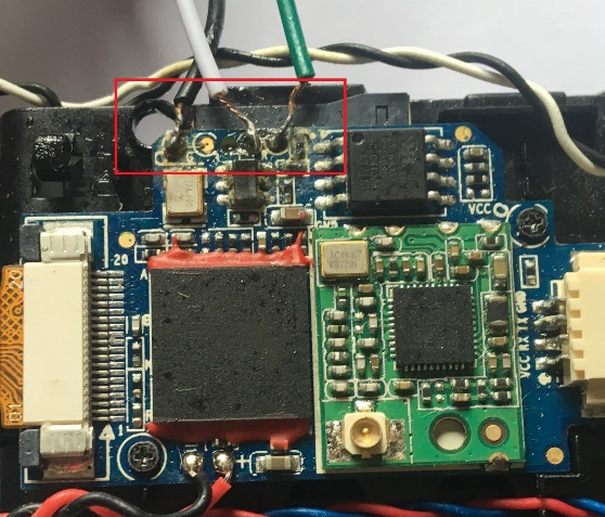
\includegraphics[width=\linewidth]{uart-pins-2}
  \caption{Good set of \acrshort{uart} pins of the Flitt Selfie Cam}
  & There were fortunately four more pins, with G, T and R tags on the side to which nothing seemed to be connected. I made sure that the G tagged pin was indeed the ground by checking the continuity between it and a known ground point on the drone with a multimeter. I then soldered my wires, connected the serial cables (Rx from the computer-side with Tx, and vice-versa). The console port of the card turns out to use a baud rate of 115,200 bauds, 8-bit data, no parity and a stop bit (abbreviated as 115200 8N1), as shown in Figure \ref{fig:uart-putty-session} when using PuTTY on Windows. Hardware flow control must be disabled. \\
\end{tabular}
\end{center}
\end{figure}

\begin{figure}[H]
  \centering
  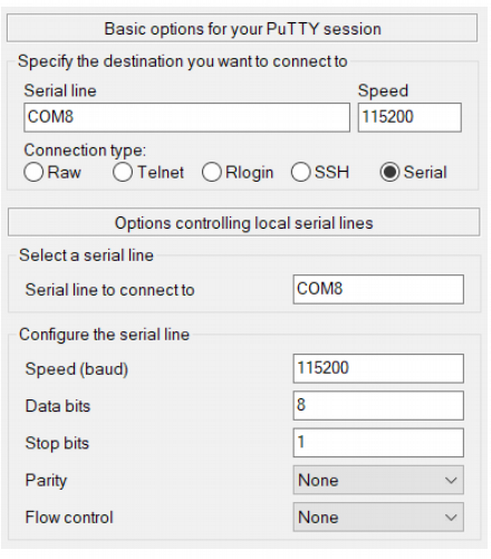
\includegraphics[width=.5\linewidth]{uart-putty-session}
  \caption{PuTTY parameters for opening a session through the \acrshort{uart}}
  \label{fig:uart-putty-session}
\end{figure}

Finally, when the connection to the serial port via \acrshort{uart} is established. A Linux-based startup sequences is displayed and, and we automatically have a root shell access to the drone !

\begin{figure}[H]
  \centering
  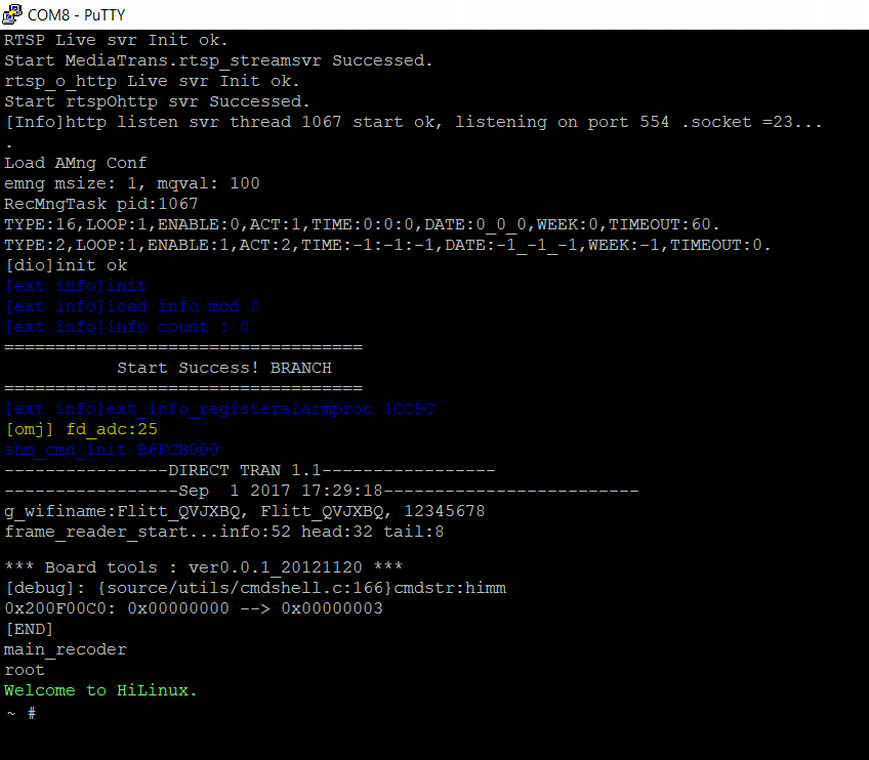
\includegraphics[width=\linewidth]{uart-shell-access-success}
  \caption{Success in getting shell access through the \acrshort{uart} on the Flitt}
  \label{fig:uart-shell-access-success}
\end{figure}

Having a shell available, it was easy to easy to recover the hash of the root password in the \texttt{/etc/passwd} file : 

\begin{center}
\begin{minipage}{.95\linewidth}
\begin{lstlisting}
root:$1$dfU0W8J6$vKtbAXdyZmq5GbYveqnnJ.:0:0::/root:/bin/sh
\end{lstlisting}
\end{minipage}
\end{center}

After analyzing the hash with the hash-identifier tool from Kali Linux, we were able to identify it as being a MD5, as shown in Figure \ref{fig:hash-identifier-root}.

\begin{figure}[H]
  \centering
  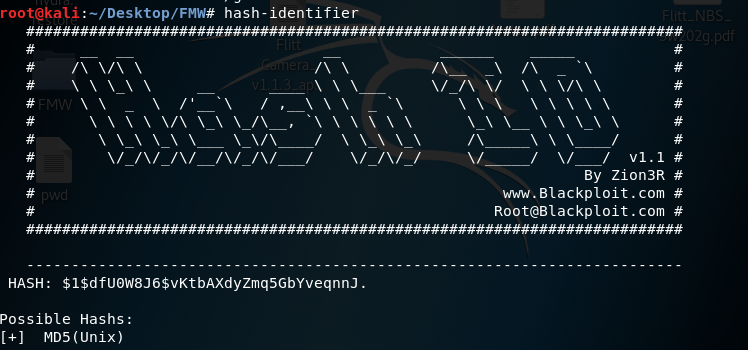
\includegraphics[width=.75\linewidth]{hash-identifier-root}
  \caption{Identifying the root password has as a MD5}
  \label{fig:hash-identifier-root}
\end{figure}

Finally, with the help of Johnny (a graphical version of the cracking program John the Ripper), and the \texttt{rockyou.txt} dictionary, we were able to crack the hash in a few minutes and therefore obtain the root password : \textbf{\texttt{ev1324}} (as shown in Figure \ref{fig:johnny-root-password}).

\begin{figure}[H]
  \centering
  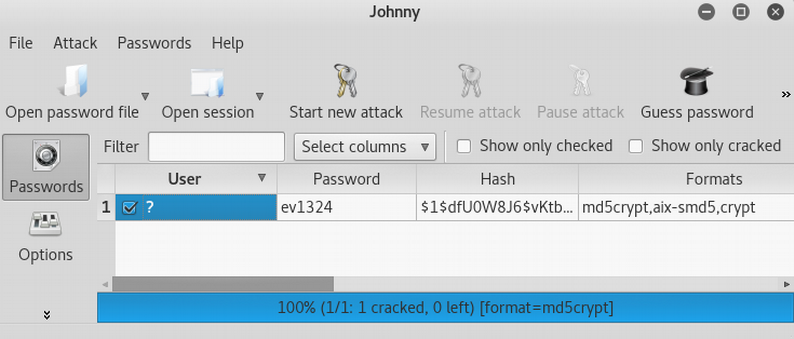
\includegraphics[width=.85\linewidth]{johnny-root-password}
  \caption{Recovering the root password}
  \label{fig:johnny-root-password}
\end{figure}

The password allowed to successfully connect to the drone with telnet, it was therefore not necessary anymore to access through the serial method.

\begin{tip}
As can be seen here, the password is the 8240422\textsuperscript{th} on the Rockyou list. It would therefore have taken roughly 34 days and 8 hours before we could successfully carry out the Telnet dictionary attack. And this is considering that we were lucky enough to guess the right user being root.

\begin{center}
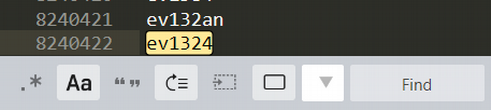
\includegraphics[width=.5\linewidth]{figures/rockyou-root-password}
\end{center}
\end{tip}

\section{C-me Selfie Drone}

This section details a few successful exploits that could be achieved.

\subsection{\acrshort{uart} shell access}

Strong with the knowledge acquired on the Flitt Selfie Cam, we applied the same technique to the C-me Selfie Drone.

\begin{figure}[H]
\begin{center}
\begin{tabular}{m{9cm}m{8.3cm}}
  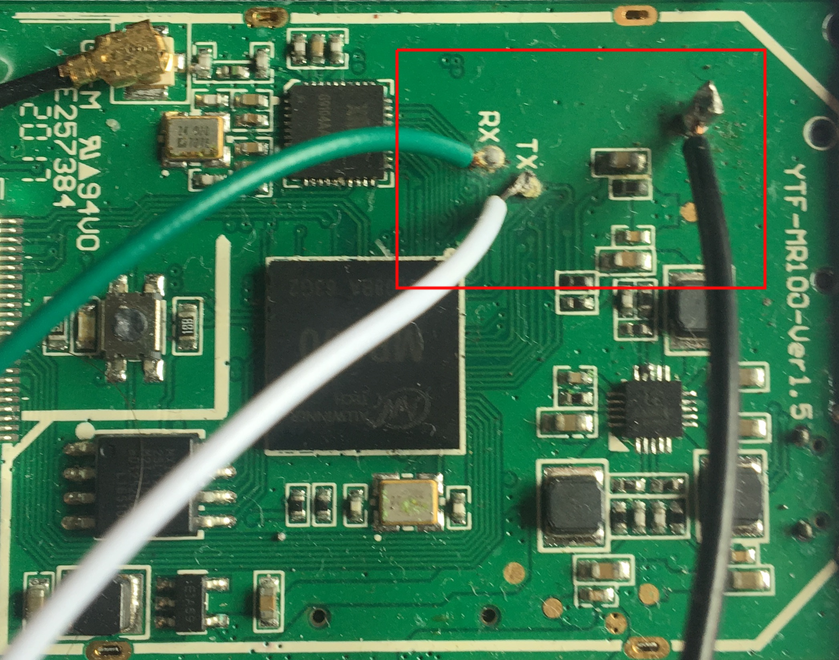
\includegraphics[width=\linewidth]{uart-rx-tx-pins}
  \caption{Set of \acrshort{uart} pins of the C-me Selfie Drone}
  & After opening the device, we quickly noticed unused connectors tagged with Rx and Tx. Therefore, it only remained to find a Ground spot using a multimeter and to proceed soldering the wires. \\
\end{tabular}
\end{center}
\end{figure}

\vspace{-1cm}
And using once again the same process, trough putty and a serial connection, we could obtain a root shell on the drone.

\begin{figure}[H]
  \centering
  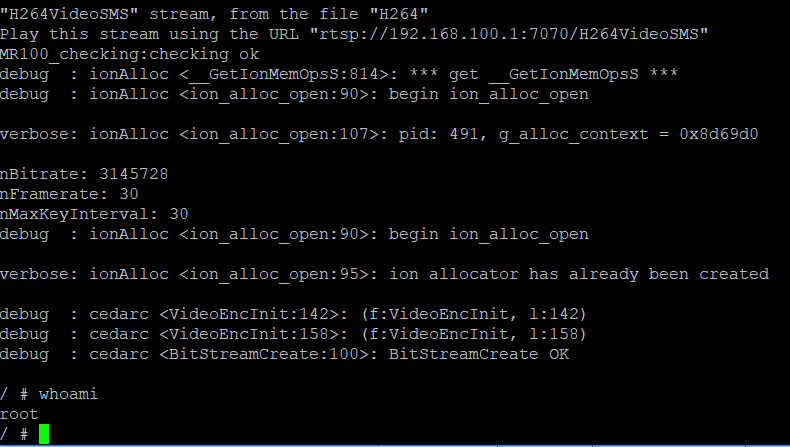
\includegraphics[width=.95\linewidth]{uart-shell-access-success-2}
  \caption{Success in getting shell access through the \acrshort{uart} on the C-me}
  \label{fig:uart-shell-access-success-2}
\end{figure}

The goal of the procedure was to gather information on the firmware from the device so that it could be reverse engineered in order to identify the services running and software vulnerabilities. Additionally, the activation of a remote management service was desirable in order to provide elevated privileges to the end-user, but couldn’t be done in an easy way since the filesystem was writing protected. This will be developed in the post-exploitation section.

\subsection{Sending config commands}\label{subsec:sending-config-commands}

Using the same procedure as in Subsection \ref{subsec:reverse-engineering}, we proceeded to change some drone's configuration, such as the WiFi password, and capture the resulting packets.

By analyzing the packets, we were able to establish that those commands are sent to the port TCP/4646, and have the syntax as shown on Figure \ref{fig:config-command}.

\begin{figure}[H]
  \centering
  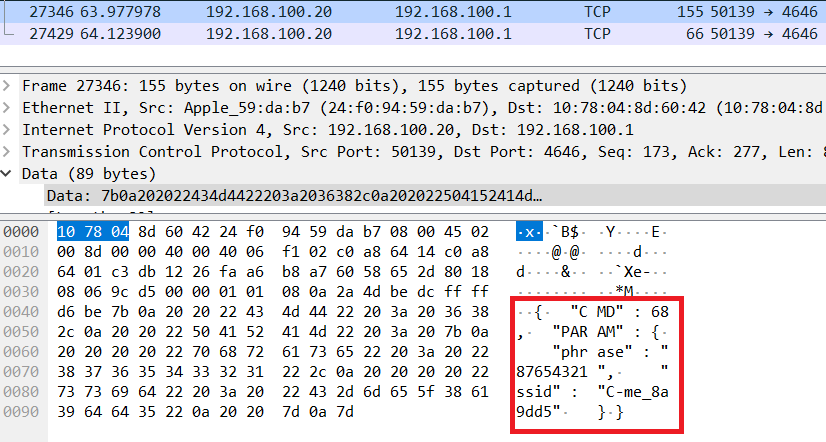
\includegraphics[width=\linewidth]{figures/config-command}
  \caption{Result of a configuration command viewed in Wireshark}
  \label{fig:config-command}
\end{figure}

And logically, we could identify the \texttt{CMD\_REQ\_NET\_PASSWORD} being the 69\textsuperscript{th} element of the enumeration discovered earlier in the config file present within the code of the APK. From here, we should be able to forge some equivalent packets in order to hack the drone.

\subsection{Post-exploitation}\label{subsec:post-exploitation}

Not being able to write on the C-me filesystem was problematic, as we felt close to our goal, getting persistent access to a shell from a distance.

Fortunately, the drone had a firmware update feature that is triggered from the smartphone application. Moreover, the only two directories that could be written on the device were obviously the \texttt{/mnt}, on which was mounted the SD card, but also a directory name \texttt{/netPrivate}. After investigation, the \texttt{/netPrivate} folder contained a specific file, named \texttt{config.dat}, that only consisted in a list of values, seeming to match the drone’s current configuration. 

Having done the update of the firmware previously without much notice, the drone was up-to-date (at version 0.7.15). It was thus no longer possible to trigger an update from the smartphone, and then to capture the traffic exchanged in order to reverse the update process.

Conveniently, in the list of values found in the \texttt{config.dat} file, one of the values matched "\texttt{0.7.15}", and since it was possible to write in the file, we proceeded to change the value to "\texttt{0.7.14}" to see if it made any difference. It did ! We were once again prompted with a message on the smartphone asking if we wanted to do a firmware update (even though the firmware was already up-to-date on the drone, we thus simply tricked the system into believing that it was not). This allowed us to capture the packets exchanged while a firmware update was happening, the same way as detailed in Subsection \ref{subsec:traffic-analysis}.

By studying the packets in Wireshark, and searching for the FTP protocol, we were able to use the functionality "\textit{follow the TCP stream}" and to uncover the whole sequence of FTP commands necessary to send a new firmware to the drone, as depicted in Figure \ref{fig:ftp-tcp-stream}. Then together with a specific control command (identification number 71) as shown in Figure \ref{fig:config-command}, we could trigger the update of drone's OS.

\begin{figure}[H]
  \centering
  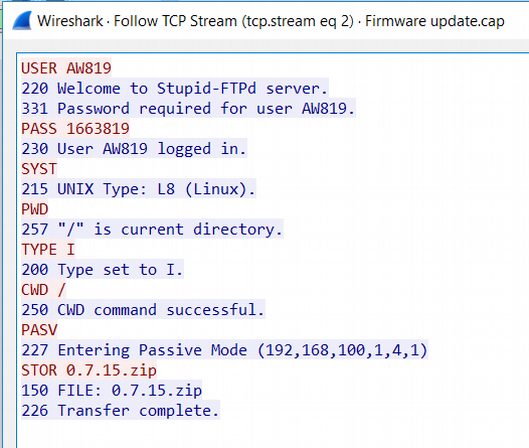
\includegraphics[width=.6\linewidth]{figures/ftp-tcp-stream}
  \caption{TCP stream of an FTP update transfer session on the C-me Selfie Drone}
  \label{fig:ftp-tcp-stream}
\end{figure}

We could also recover the \texttt{0.7.15.zip} file containing the firmware. From this point, we were now able to update the firmware of the drone from our computers.

Inside the archive, a file named \texttt{rootfs.squashfs} was present. SquashFS \cite{squashfs} is an open source, read only, extremely compressible filesystem. The SquashFS filesystem tools come in a separate package. This package is called \texttt{squashfs-tools} \cite{squashfs-tools}. Once installed, it is possible to open the file and inside can be found the entire filesystem of the C-me drone !

At this point, we were able to locate a script in \texttt{/etc} named \texttt{autorun.sh} that is used to launch a set of services at boot time. We thus simply added a line having the effect of launching the Telnet service and re-created the archive.

Once the new modified firmware was uploaded, the telnet service was running on the drone from the boot and we could connect to it with the root user via Telnet. We now have created a backdoor on the device !

\begin{summary}
The \textbf{exploitation} is probably the \textbf{most rewarding step} of all the pentesting process. Indeed, this is the moment when the attacker put to the test the vulnerabilities found in the previous phases to advance in the intrusion of the information system. Obviously, the outcome of the exploitation phase is highly dependent on the quality of the research already achieved.

\textbf{Two} different \textbf{scenarios} are possible at this stage :
\begin{itemize}
  \item Either you have uncovered an already \textbf{known vulnerability} that can be \textbf{exploited with a tool} or an attack that is usable with few efforts.
  \item Either there is a vulnerability, but it is up to the attacker to \textbf{come with an innovative solution} that can either be a piece of code or a clever use of an existing tool.
\end{itemize}

During the process of our exploitation phase we were brought to put into direct practice the latest statement. Indeed, \textbf{some exploits were} rather \textbf{straightforward}, with many examples in the literature and therefore consisted more in a technical execution, but some others had to be forged by us.

In short, on the \textbf{Flitt Selfie Cam} we carried out a dictionary attack in an attempt to crack the telnet credentials. Being unsuccessful, we opted to open the device and perform a hardware hacking of the \acrshort{uart} serial line. This resulted in obtaining a \textbf{root shell} access to the OS. From within, it was therefore possible to crack the root account’s password through its hash. Once the \textbf{password uncovered}, we had direct access on the drone thanks to the \textbf{Telnet} service.

On the \textbf{C-me Selfie Drone}, we first tried to exploit the FTP service without any luck. Then, strong with the hardware hack knowledge and success gained on the Flitt, we applied once again the same procedure with the \textbf{same outcome} on the C-me. Once inside, we could establish that a Telnet service was indeed installed on the drone but not running by default. Unfortunately, impossible to write anything on the filesystem except for the \texttt{/mnt} repository, as it was protected.

Finally, on \textbf{both drones}, we were able to \textbf{forge configuration commands}, through python scripts, that allowed us to change critical information on the drones, such as the \acrshort{ssid} or the WiFi password ; as well as deleting the video media or even shutting it down.

Not giving up on the \textbf{C-me Selfie Drone}, we managed to understand how the \textbf{firmware update} process was working and were able to forge our own firmware in which the telnet service was activated. Once updated, the drone therefore contained a \textbf{backdoor} that we could then exploit a our advantage, thus adding a post-exploitation component to our whole process.
\end{summary}

\begin{discussion}
Once the reconnaissance and vulnerability analysis phases are completed, the pentester should have a more thorough understanding of his target. At this point, a list of weaknesses and possible attack vectors allows him to plan which attack has the higher chances to succeed.

In our process, we naturally focused first on attacks that were involving automated tools to be carried out. For instance, a dictionary attack on the telnet server of the Flitt or some tries to make usage of some Metasploit’s built in exploits on the FTP server of the C-me or directly on the Linux OS of the drones.

But after as many failures as there were attempts, the hope of success was shrinking quickly and one could ask if we were really up to the task.

Later, by checking know hacks in the scope of the Hi3518 chip (which is the main chip of the Flitt and is commonly used on light video devices), we stumbled upon a methodology allowing to obtain root shell access on an IP camera that was base on the same chip. Though it was some hardware hacking.

Initially, we didn’t consider hardware hacking as part of the scope of the work, but having no better alternative at this point we decided to apply the described methodology to the drone. 
In order to perform this hack, the attacker has to physically connect wires to an UART serial line eventually left unprotected by the manufacturer. We would like to express our gratitude to Ir Valéry Broun for devoting his precious time to the soldering of the necessary wires.

The hack didn’t succeed on the first try, notably because there were more than one serial line on the PCB, but after a week of trying and a steep soldering learning curve, we finally managed to obtain a shell access to the drone’s OS.

Strong with the former experience, the hack was quickly repeated on the C-me drone, following the exact same methodology. We might have uncovered a pattern to hack light video drones
From this point, we were able to dig into the OS of both devices, and finally take full advantage of all the information gathered during the reconnaissance and vulnerability analysis phases.

As Kevin Mitnick stated, there is always a hole to break into a system. We learned from this experience that the key to success is, after knowledge, perseverance.
\end{discussion}

\end{chaptercover}
